\section{Vision Transformers}
\begin{frame}{}
    \LARGE Vision Transformers: \textbf{The ViT Architecture}
\end{frame}

\begin{frame}{Vision Transformer (ViT) Architecture}
    \textbf{Key idea:}
    \begin{itemize}
        \item Split image into fixed-size patches (e.g., 16$\times$16)
        \item Flatten and project patches into embeddings
        \item Add positional encodings to embeddings
        \item Apply standard Transformer encoder
    \end{itemize}
    \vspace{0.5em}
    \textbf{Architecture:}
    \begin{itemize}
        \item Patch embedding
        \item Class token
        \item Transformer blocks
        \item MLP Head
    \end{itemize}
    {\footnotesize\textit{Source: Dosovitskiy et al., ``An Image is Worth 16x16 Words'', 2020}}
\end{frame}

\begin{frame}{Vision Transformers}
\only<1>{
\begin{figure}
\centering
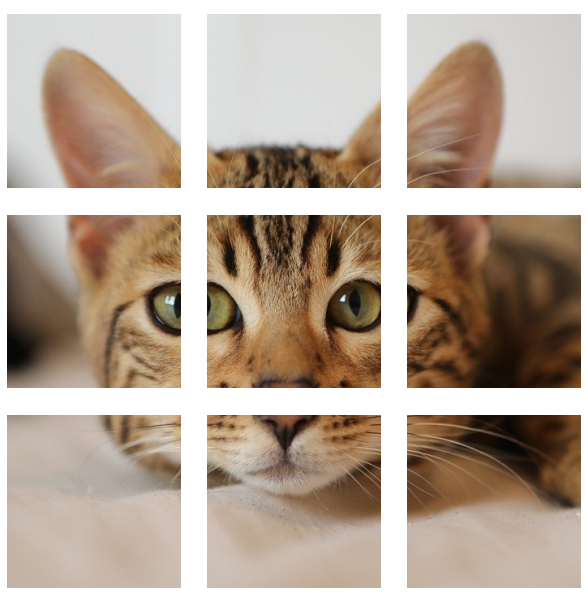
\includegraphics[width=1.0\textwidth,height=0.82\textheight,keepaspectratio]{images/advanced-cv/vit_1.png}
\caption*{\tiny Source: UMich EECS 498 (2022), Lecture 18: Vision Transformers, slide 52}
\end{figure}
}

\only<2>{
\begin{figure}
\centering
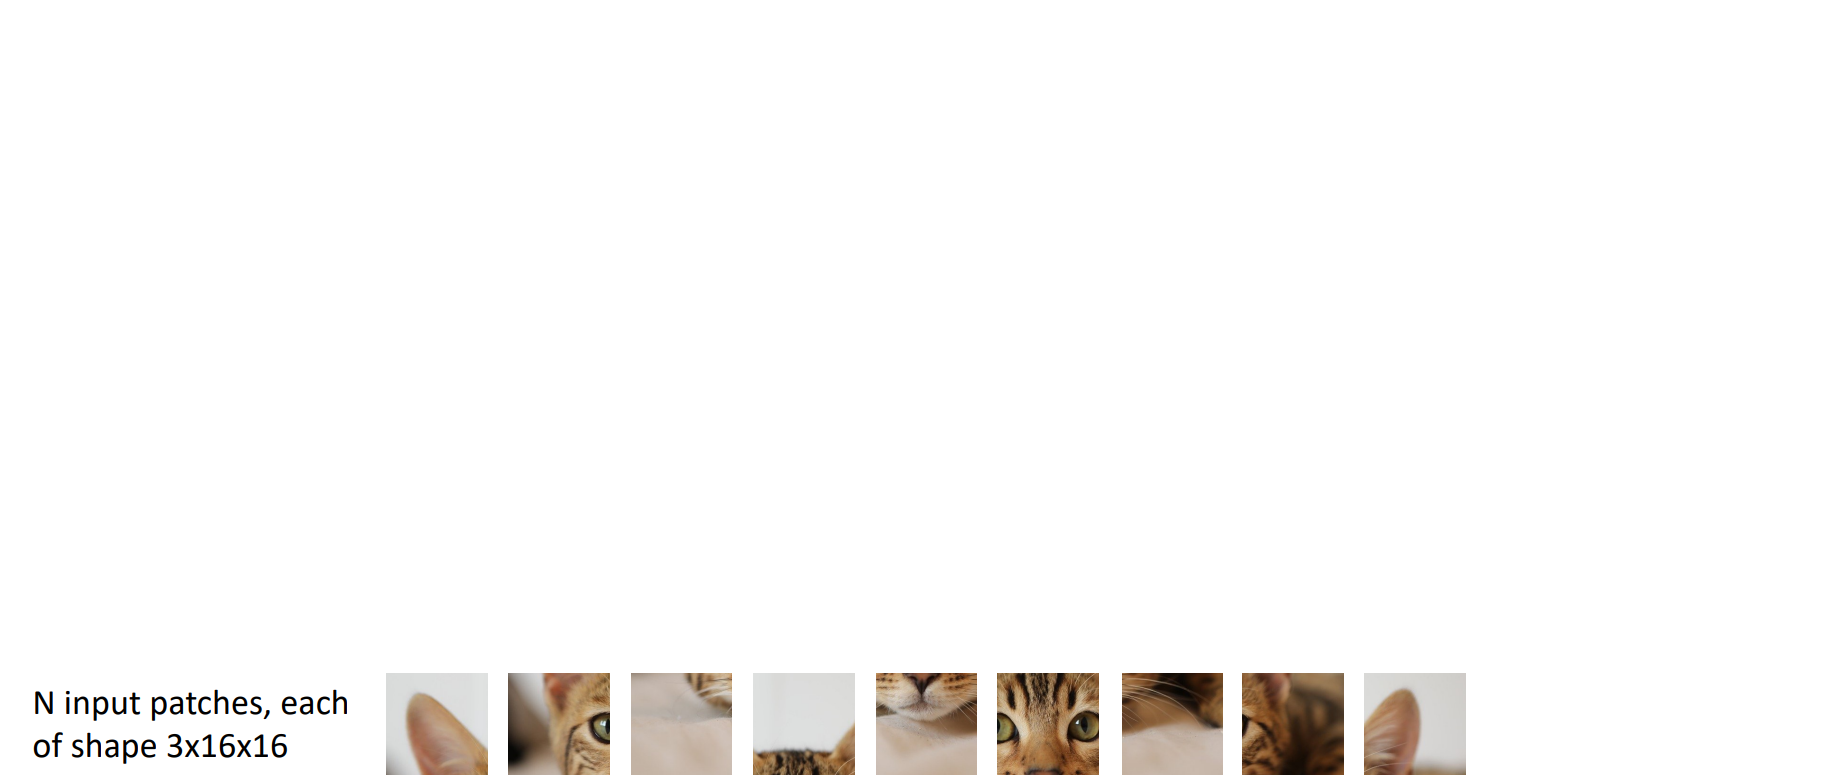
\includegraphics[width=1.0\textwidth,height=0.88\textheight,keepaspectratio]{images/advanced-cv/vit_2.png}
\caption*{\tiny Source: UMich EECS 498 (2022), Lecture 18: Vision Transformers, slide 53}
\end{figure}
}

\only<3>{
\begin{figure}
\centering
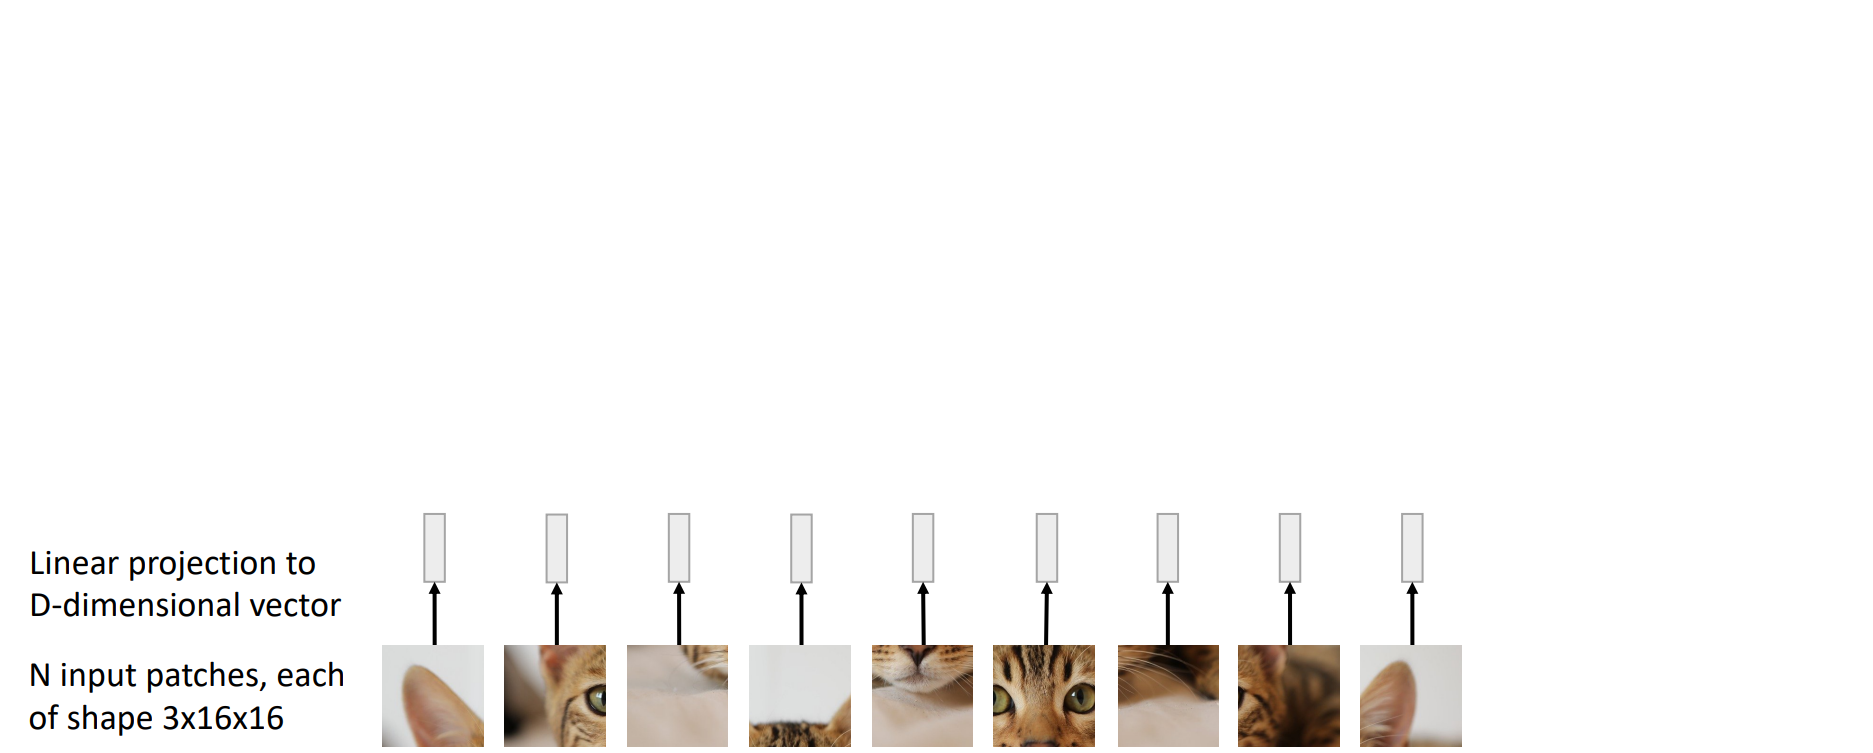
\includegraphics[width=1.0\textwidth,height=0.88\textheight,keepaspectratio]{images/advanced-cv/vit_3.png}
\caption*{\tiny Source: UMich EECS 498 (2022), Lecture 18: Vision Transformers, slide 54}
\end{figure}
}

\only<4>{
\begin{figure}
\centering
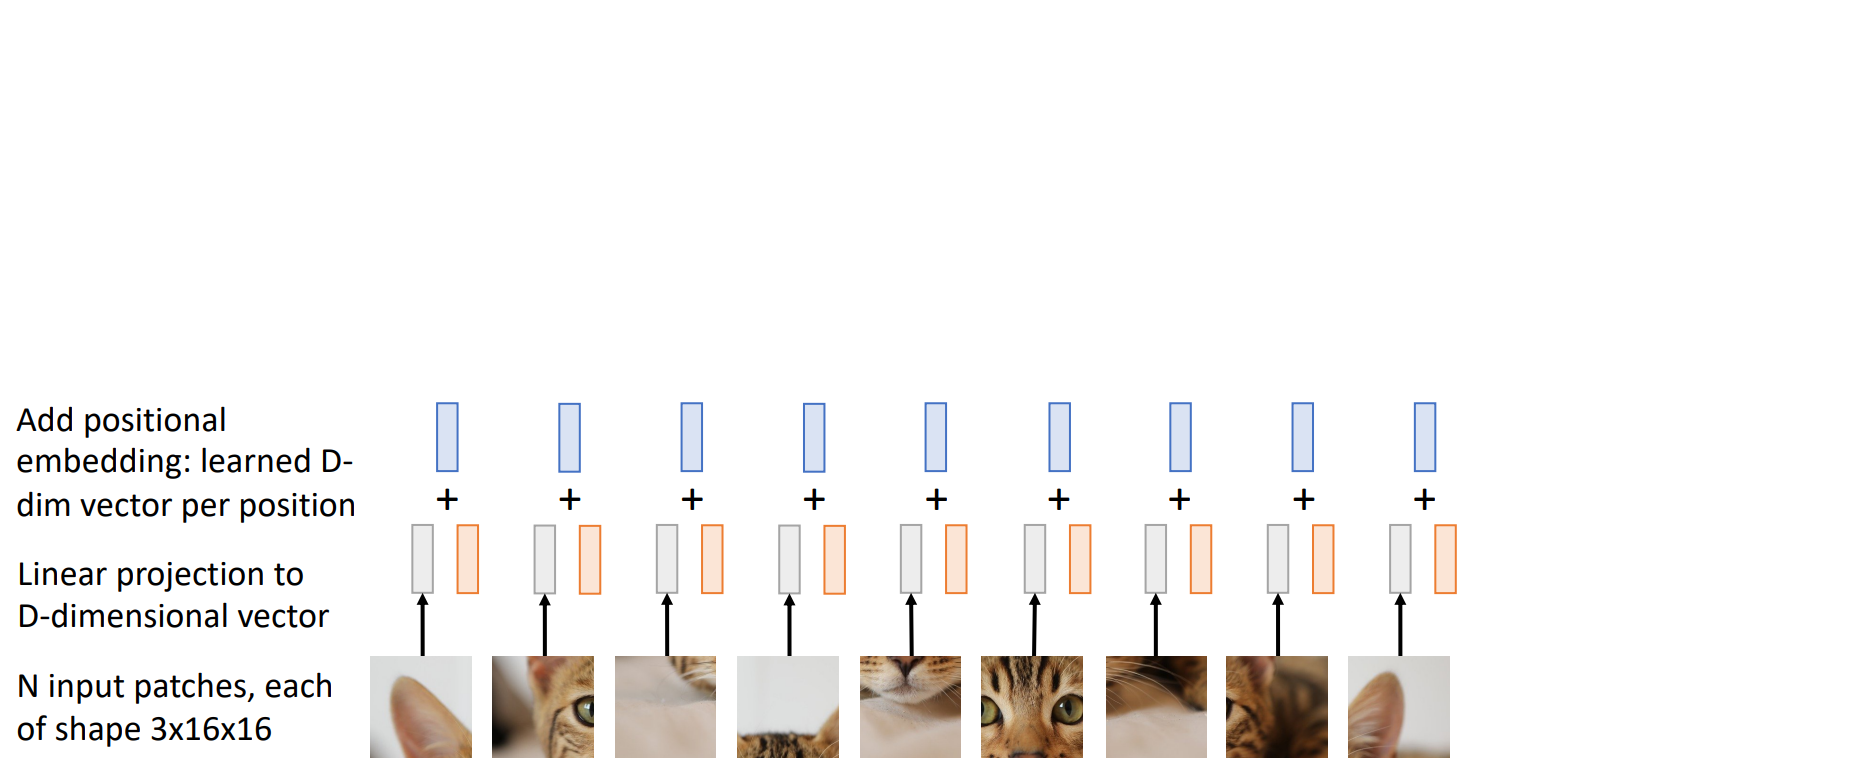
\includegraphics[width=1.0\textwidth,height=0.88\textheight,keepaspectratio]{images/advanced-cv/vit_4.png}
\caption*{\tiny Source: UMich EECS 498 (2022), Lecture 18: Vision Transformers, slide 55}
\end{figure}
}

\only<5>{
\begin{figure}
\centering
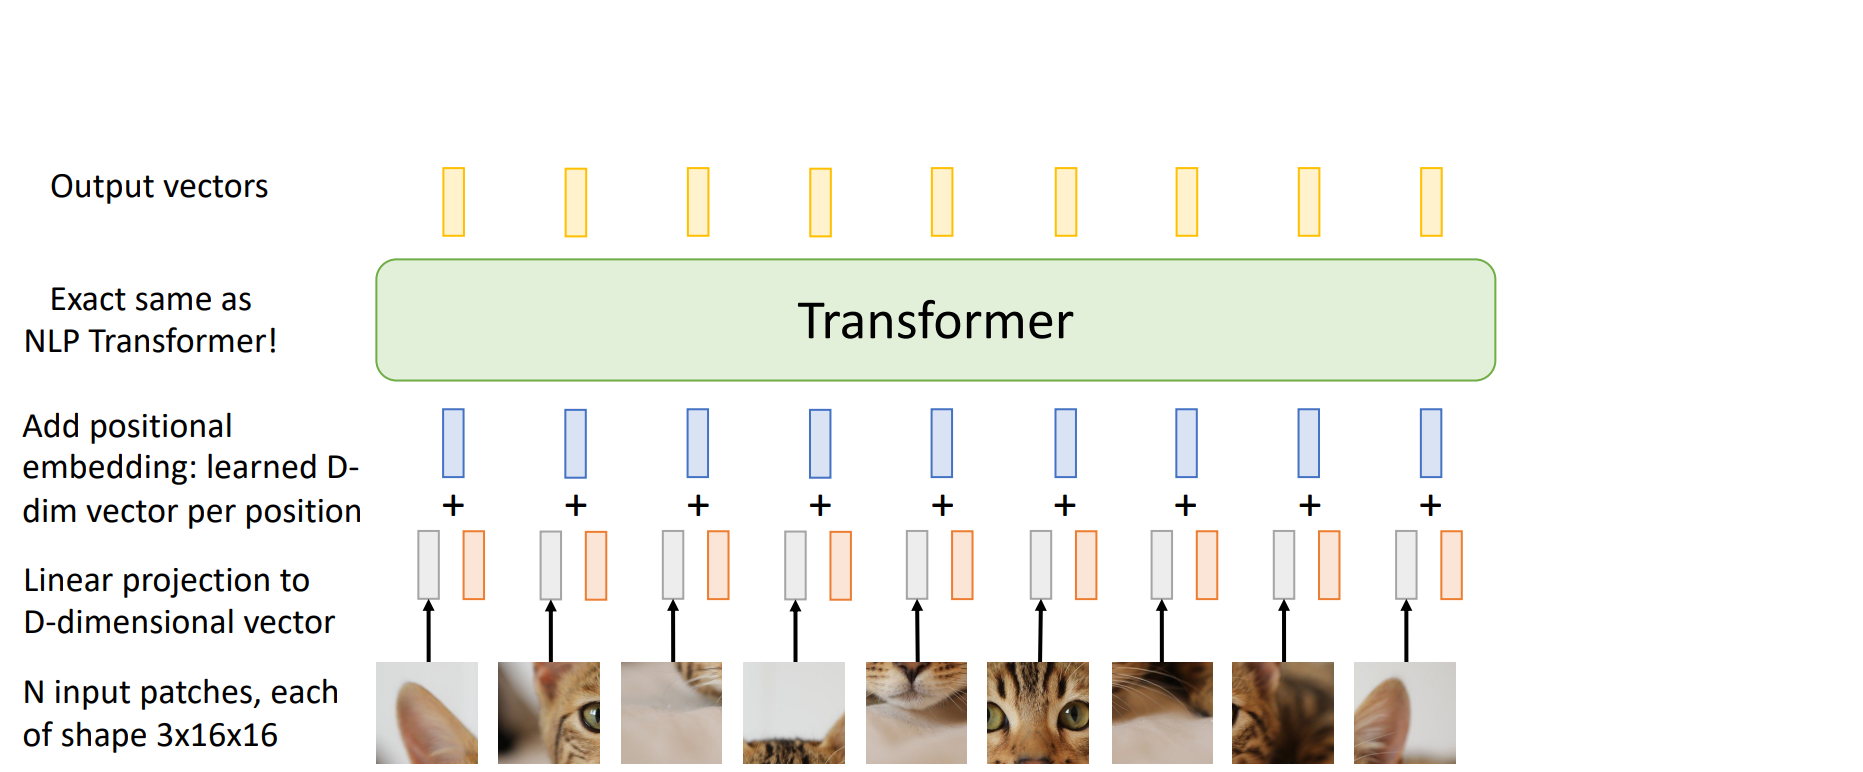
\includegraphics[width=1.0\textwidth,height=0.88\textheight,keepaspectratio]{images/advanced-cv/vit_5.png}
\caption*{\tiny Source: UMich EECS 498 (2022), Lecture 18: Vision Transformers, slide 56}
\end{figure}
}

\only<6>{
\begin{figure}
\centering
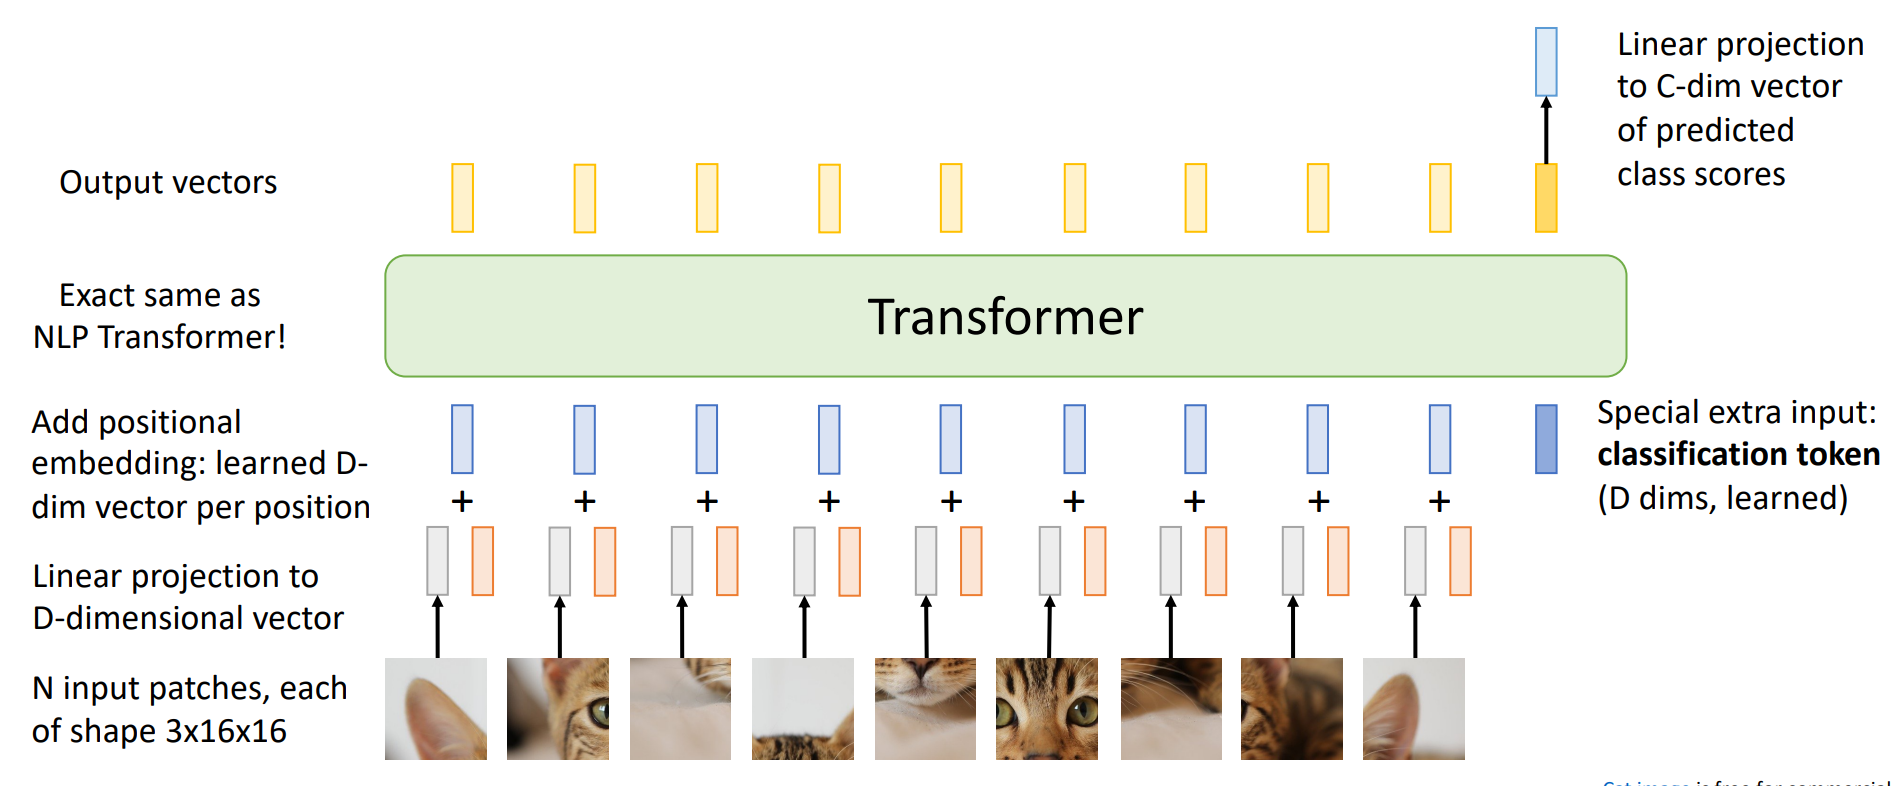
\includegraphics[width=1.0\textwidth,height=0.88\textheight,keepaspectratio]{images/advanced-cv/vit_6.png}
\caption*{\tiny Source: UMich EECS 498 (2022), Lecture 18: Vision Transformers, slide 58}
\end{figure}
}

\only<7>{
\begin{figure}
\centering
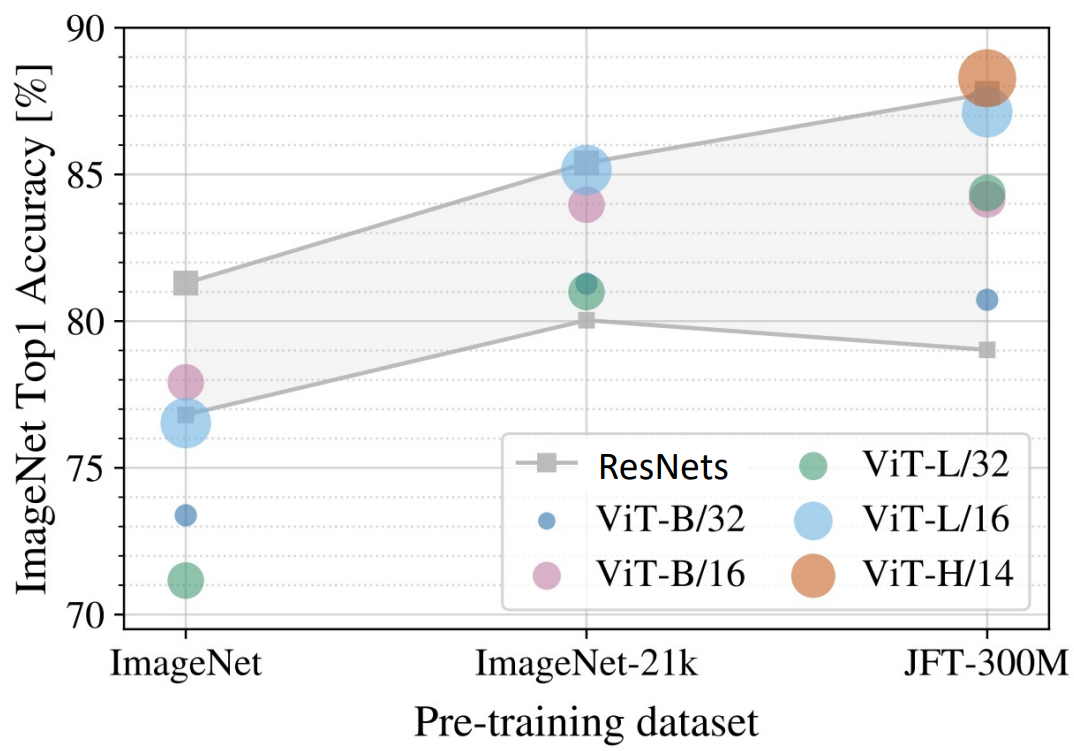
\includegraphics[width=1.0\textwidth,height=0.9\textheight,keepaspectratio]{images/advanced-cv/vit_7.png}
\end{figure}  
\footnotetext{Dosovitskiy et al, “An Image is Worth 16x16 Words: Transformers for Image Recognition at Scale”, ICLR 2021}

}

\end{frame}